%General Physics IIA Homework_8
\documentclass[10pt,a4paper]{article}
\usepackage[UTF8]{ctex}
\usepackage{bm}
\usepackage{amsmath}
\usepackage{extarrows}
\usepackage{amsthm}
\usepackage{amssymb}
\usepackage{graphicx}
\title{General Physics Homework\_{}8}
\author{陈稼霖 \and 45875852}
\date{2018.6.4}
\theoremstyle{remark}
\newtheorem{defi}{Definition}
\newtheorem{cdefi}{\bf 定义}
\begin{document}
\maketitle
\section{}
\subsection{解:}
当一个交流电$I = I_0\cos(\omega t)$通过这个线圈,不妨先设交流电垂直穿过这一圆形线圈的中心(当然,$V(t)$与线圈的具体形状和交流电穿过的具体位置无关,这在(2)中将会证明)。由于线圈的长度$L^2\gg A$,故可近似认为,交流电在线圈的小圆环处产生的磁场是均匀的,根据$Biot-Savart$ 定律,交流电在线圈的小圆环处产生的磁场为
\[
BL = \mu_0I
\]
\[
\Rightarrow B(t) = \frac{\mu_0I}{L} = \frac{\mu_0I_0\cos(\omega t)}{L}
\]
对应通过线圈的总磁通量为
\[
\Phi(t) = NB(t)A = \frac{N\mu_0I_0A\cos(\omega t)}{L}
\]
根据电磁感应定律,线圈两端的感应电压为
\[
V(t) = - \frac{d\Phi(t)}{dt} = \frac{N\mu_0\omega I_0A\sin(\omega t)}{L}
\]
\subsection{证明:}
假设线圈为任意形状,交流电$I(t)$从线圈中的任意位置通过。线圈的匝数密度(单位长度的匝数)为
\begin{equation}
\label{CoilTensity}
n = \frac{N}{L}
\end{equation}
通过线圈的总磁通量为
\[
\Phi = \oint_LBndl = \frac{N}{L}\oint_LBdl
\]
根据安培环路定理的积分形式,有
\[
\oint_LBdl = \mu_0I = \mu_0I_0\cos(\omega t)
\]
故根据电磁感应定律,线圈两端的感应电压为
\begin{equation}
\label{Magnetism}
V(t) = - \frac{d\Phi}{dt} = - \frac{d(\frac{N}{L}\mu_0I_0\cos(\omega t))}{dt} = \frac{N\mu_0\omega I_0A\sin(\omega t)}{L}
\end{equation}
故线圈两端的感应电压$V(t)$与线圈的具体形状和交流电$I(t)$穿过的具体位置没有关系。
\subsection{答:}
返回的导线必须要穿过线圈中心是因为,导线的螺旋部分可以在垂直于线圈所在平面方向(即垂直于纸面方向)上产生磁场,这一磁场分量的大小等于一个长度为$L$,且形状与线圈螺旋部分的轴线相同的单匝线圈产生的磁场,这一磁场分量的变化可以改变线圈的磁通量,感应出额外的感应电动势,从而影响线圈两端的电压,造成误差;而使返回的导线穿过线圈中心,则返回的导线所产生的磁场恰好可以抵消这一方向的磁场分量,使线圈在垂直其所在平面方向(即垂直于纸面方向)上磁感应强度为$0$,避免产生多余的感应电动势,从而减小测量的误差。
\subsection{答:}
这个装置可能的主要误差来源有:

(1)由于将交流电在线圈的同一个小圆环中不同点产生的磁场近似视为均匀,造成的误差,这一近似得到的线圈两端电压理论值比其实际值要小;

(2)由于线圈的匝数密度不均匀导致的式(\ref{CoilTensity})不适用,从而产生误差;

(3)根据楞次定律,为了阻碍通过自身的磁通量的变化,当通过线圈的交流电增大时,线圈有一种向外扩张的趋势,当通过线圈的交流电减小时,线圈有一种向内收缩的趋势,故若线圈由硬度不太大的材料制成且不加以固定,很容易在通过交流电时造成线圈的形变从而改变其磁通量变化情况,从而影响到线圈两端的感应电压,造成误差;

(4)线圈各参数(如线圈长度$L$、线圈横截面积$A$)的测量值与其真值的误差,导致通过式(\ref{Magnetism})计算时产生的误差;

(5)线圈存在自感,即线圈中的感应电流也可以产生变化的磁场,并感应出额外的感应电动势,造成误差。
\section{}
\subsection{解:}
设通过电阻$R$所在支路的电流为$I_1(t)$,通过电感$L$所在支路的电流为$I_2(t)$,通过电容$C$ 所在支路的电流为$I_3(t)$。则对于三条支路与电源组成的回路,根据电磁感应定律分别有
\[
\left\{\begin{array}{l}
- E_0\cos \omega t + RI_1 = 0\\
- E_0\cos \omega t = - L\frac{dI_2}{dt}\\
- E_0\cos \omega t + \frac{\int I_3dt}{C} = 0
\end{array}\right.
\]
又考虑到当$t=0$的初始状态下
\[
\left\{\begin{array}{l}
I_1(0) = \frac{E_0}{R}\\
E_0 = L\frac{dI_2}{dt}(0)\\
I_3(0) = 0
\end{array}\right.
\]
解得
\[
\left\{\begin{array}{l}
I_1(t) = \frac{E_0}{R}\cos \omega t\\
I_2(t) = \frac{E_0}{\omega L}\sin \omega t\\
I_3(t) = -\omega CE_0\sin \omega t
\end{array}\right.
\]
故干路上的总电流为
\[
\begin{split}
I = I_1 + I_2 + I_3 = \frac{E_0}{R}\cos \omega t + \frac{E_0}{\omega L}\sin \omega t-\omega CE_0\sin \omega t\\
= \sqrt{(\frac{1}{R})^2+(\frac{1}{\omega L}-\omega C)^2}E_0\cos(\omega t + \varphi)
\end{split}
\]
其中$\tan\varphi = \frac{\omega C-\frac{1}{\omega L}}{\frac{1}{R}}$。故干路电流的幅值与频率之间的关系即
\[
I_0(\omega) = \sqrt{(\frac{1}{R})^2+(\frac{1}{\omega L}-\omega C)^2}E_0
\]
设$R = 1\Omega,L = 1H,C = 1F,E_0 = 1V$,以干路电流频率$\omega$为横坐标,以干路电流幅值$I_0(\omega)$为纵坐标,作$I_0\sim\omega$曲线如图\ref{I_0omega curve of LRC parallel connection circuit}。
\begin{figure}
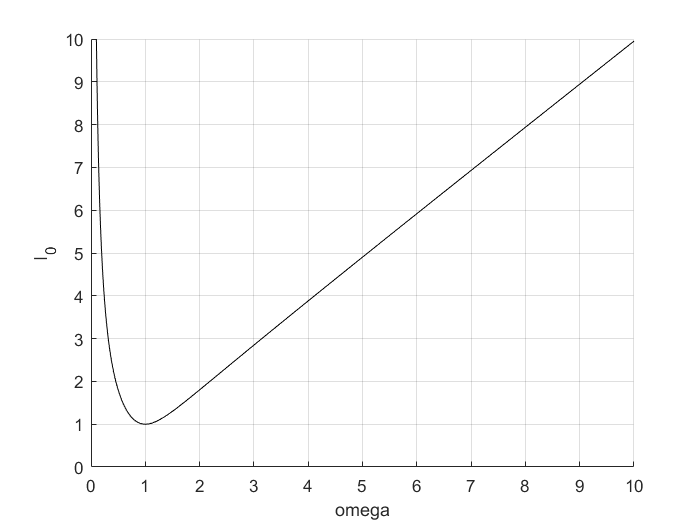
\includegraphics[scale = 0.6]{Fig_1.png}
\caption{LRC并联电路中干路电流幅值随电源电压频率变化曲线}
\label{I_0omega curve of LRC parallel connection circuit}
\end{figure}
\subsection{解:}
对于$R = K\sqrt{\frac{L}{C}}$且$K\gg 0$的$RLC$并联电路,当电源电压频率$\omega = \frac{1}{\sqrt{LC}}$时,干路电流幅值达到最小值${I_0}_{min} = \frac{E_0}{R}$,当电路的干路电流幅值达到其最小值的$\sqrt{2}$倍时,有
\[
I_0(\omega) = \sqrt{(\frac{1}{R})^2+(\frac{1}{\omega L}-\omega C)^2}E_0 = \sqrt{2}{I_0}_{min} = \frac{\sqrt{2}E_0}{R}
\]
解得对应的电源电压频率为
\[
\omega_{\pm} = \frac{\pm\frac{1}{R} + \sqrt{\frac{1}{R^2} + \frac{4C}{L}}}{2C} = \frac{\pm1 + \sqrt{1+4K^2}}{2K\sqrt{LC}}
%\xlongequal{K\gg 0}\frac{1}{\sqrt{LC}}
\]
%\[
%\begin{split}
%\omega_{\pm} &= \sqrt{\frac{(\frac{3}{R^2}+\frac{2C}{L})\pm \sqrt{\frac{3}{R^2}(\frac{3}{R^2}+\frac{4C}{L})}}{2C^2}} = \sqrt{\frac{(\frac{3}{R^2C^2}+\frac{2}{LC})\pm\sqrt{\frac{9}{R^4C^4}+\frac{12}{LC^3}}}{2}}\\
%&= \sqrt{\frac{(\frac{3}{KLC}+\frac{2}{LC})\pm\sqrt{\frac{9}{K^2L^2C^2}+\frac{12}{LC^3}}}{2}}\\
%&\begin{array}{c}
%K\gg 0\\
%=====
%\end{array}
%\sqrt{\frac{1}{LC}\pm\frac{1}{C}\sqrt{\frac{3}{LC}}}
%\end{split}
%\]
故其谐振曲线频带宽度为
\[
\Delta\omega = \omega_ + -\omega_- = \frac{1 + \sqrt{1+4K^2}}{2K\sqrt{LC}} - \frac{- 1 + \sqrt{1+4K^2}}{2K\sqrt{LC}} = \frac{1}{K\sqrt{LC}}
\]
而对于$R = \frac{1}{K}\sqrt{\frac{L}{C}}$且$K\gg 0$的$RLC$串联电路,设电流为$I(t)$。 则对于电源与$LRC$组成的回路,根据电磁感应定理有
\begin{equation}
\label{SeriesConnection}
- E_0\cos\omega t + RI_0\cos\omega t + \frac{\int I_0dt}{C} = - L\frac{dI_0}{dt}
\end{equation}
设电源电压的复数形式为$\widetilde{E(t)} = E_0e^{i\omega t}$,设电流的复数形式为$\widetilde{I(t)} = I_0e^{i\omega t}$,则
\[
\left\{\begin{array}{l}
E(t) = Re(\widetilde{E(t)})\\
I(t) = Re(\widetilde{I(t)})
\end{array}\right.
\]
则(\ref{SeriesConnection})中的公式可化为
\[
Re(- \widetilde{E} + R\widetilde{I} + \frac{\int\widetilde{I}dt}{C}) = Re(- L\frac{\widetilde{I}}{dt})
\]
\[
\Rightarrow(R + \frac{1}{i\omega C} + i\omega L)\widetilde{I} = E_0e^{i\omega t}
\]
\[
\Rightarrow \widetilde{I} = \frac{E_0e^{i\omega t}}{R + \frac{1}{i\omega C} + i\omega L}
\]
\[
\Rightarrow \widetilde{I} = \frac{E_0e^{i(\omega t + \phi)}}{\sqrt{R^2 + (\frac{1}{\omega C} - \omega L)^2}}
\]
其中$\tan\phi = \frac{\frac{1}{\omega C} - \omega L}{R}$。则电流幅值为
\[
I_0 = \frac{E_0}{\sqrt{R^2 + (\frac{1}{\omega C} - \omega L)^2}}
\]
则当$\frac{1}{\omega C} - \omega L = 0$,即$\omega = \frac{1}{\sqrt{LC}}$时,电流幅值达到最大值${I_0}_{max} = \frac{E_0}{R}$,当电流幅值达到其最大值的$\frac{1}{\sqrt{2}}$ 时,有
\[
I_0 = \frac{E_0}{\sqrt{R^2 + (\frac{1}{\omega C} - \omega L)^2}} = \frac{1}{\sqrt{2}}{I_0}_{max} = \frac{E_0}{\sqrt{2}R}
\]
解得对应的电源电压频率为
\[
\omega_{\pm} = \frac{\pm\frac{1}{R} + \sqrt{\frac{1}{R^2} + \frac{4C}{L}}}{2L} = \frac{\pm1 + \sqrt{1+4K^2}}{2K\sqrt{LC}}
\]
%\[
%\begin{split}
%\omega_{\pm} &= \sqrt{(\frac{3R^2+\frac{2L}{C})\pm\sqrt{9R^4+\frac{12L}{C}}}{2L^2}} = \sqrt{\frac{(\frac{3R^2}{L^2}+\frac{2}{LC})\pm\sqrt{\frac{9R^4}{L^4}+\frac{12}{L^3C}}}{2}}\\
%&= \sqrt{\frac{(\frac{3}{KLC}+\frac{2}{LC})\pm\sqrt{\frac{9}{K^2L^2C^2}+\frac{12}{L^3C}}}{2}}\\
%&\begin{array}{c}
%K\gg 0\\
%=====
%\end{array}
%\sqrt{\frac{1}{LC}\pm\frac{1}{L}\sqrt{\frac{3}{LC}}}
%\end{split}
%\]
故其谐振曲线频带宽度为
\[
\Delta\omega = \omega_+ - \omega_- = \frac{1 + \sqrt{1+4K^2}}{2K\sqrt{LC}} - \frac{- 1 + \sqrt{1+4K^2}}{2K\sqrt{LC}} = \frac{1}{K\sqrt{LC}}
\]
两种电路的谐振频率相等$\omega = \frac{1}{\sqrt{LC}}$,且频带宽度相等$\Delta\omega = \frac{1}{K\sqrt{LC}}$。
%观察到两种电路的频带宽度公式十分相似,若$L<C$,则$LRC$并联电路的频带宽度大于$LRC$串联电路的频带宽度,若$L>S$,则$LRC$并联电路的频带宽度小于$LRC$串联电路的频带宽度,若$L>S$,则$LRC$ 并联电路的频带宽度等于$LRC$串联电路的频带宽度。
\section{}
\subsection{证明:}
设$\overrightarrow{E_0}$的$x,y,z$分量分别为$\overrightarrow{E_0} = (E_{0x},E_{0y},E_{0z})$,则$\overrightarrow{E}$的$x,y,z$分量分别为$\overrightarrow{E} = (E_{0x}e^{i(\omega t-kx)},E_{0y}e^{i(\omega t-kx)},E_{0z}e^{i(\omega t-kx)})$。则有
\[
\begin{split}
\frac{\partial^2\overrightarrow{E}}{{\partial t}^2} &= -\omega^2\overrightarrow{E_0}e^{i(\omega t-kx)}\\
&= (- \omega^2E_{0x}e^{i(\omega t-kx)},- \omega^2E_{0y}e^{i(\omega t-kx)},- \omega^2E_{0z}e^{i(\omega t-kx)})
\end{split}
\]
和
\[
\begin{split}
\nabla^2\overrightarrow{E} &= (\frac{\partial^2E_{0x}e^{i(\omega t-kx)}}{\partial^2t},\frac{\partial^2E_{0y}e^{i(\omega t-kx)}}{\partial^2y},\frac{\partial^2E_{0z}e^{i(\omega t-kx)}}{\partial^2z})\\
&= (- k^2E_{0x}e^{i(\omega t-kx)},- k^2E_{0y}e^{i(\omega t-kx)},- k^2E_{0z}e^{i(\omega t-kx)})\\
&= - k^2\overrightarrow{E_0}e^{i(\omega t-kx)}
\end{split}
\]
从而有
\[
\frac{\partial^2\overrightarrow{E}}{\partial^2t} = \frac{k^2}{\omega^2}\nabla^2\overrightarrow{E}
\]
故场$\overrightarrow{E}$满足波动方程。自然,对于场$\overrightarrow{E}$的每个分量,都有
\[
\left\{\begin{array}{l}
\frac{\partial^2E_x}{\partial^2t} = \frac{k^2}{\omega^2}\frac{\partial^2E_x}{\partial^2x}\\
\frac{\partial^2E_y}{\partial^2t} = \frac{k^2}{\omega^2}\frac{\partial^2E_y}{\partial^2y}\\
\frac{\partial^2E_z}{\partial^2t} = \frac{k^2}{\omega^2}\frac{\partial^2E_z}{\partial^2z}\\
\end{array}\right.
\]
故场$\overrightarrow{E}$的每个分量都满足波动方程。
\subsection{证明:}
$\overrightarrow{E}$的实部为
\[
Re(\overrightarrow{E}) = Re(\overrightarrow{E_0}[\cos(\omega t- kx) + i\sin(\omega t- kx)]) = \overrightarrow{E_0}\cos(\omega t- kx)
\]
坐标为$x$的点在时刻$t$的波动状态与坐标为$(x+\Delta x)$($\Delta x>0$)的点在时刻$(t+\frac{k\Delta x}{\omega})$(晚于时刻$t$)的波动状态相同,故相当于一个沿$x$ 轴传播的平面波,这波向$x$ 轴正方向传播(且速度为$\frac{\omega}{k}$)。
\subsection{证明:}
算符$\nabla$对$(a)$中的函数作用,有
\[
\begin{split}
\nabla\cdot\overrightarrow{E} &= \nabla\cdot(E_{0x}e^{i(\omega t-kx)},E_{0y}e^{i(\omega t-kx)},E_{0z}e^{i(\omega t-kx)})\\
&= \frac{\partial E_{0x}e^{i(\omega t-kx)}}{\partial x} + \frac{\partial E_{0y}e^{i(\omega t-kx)}}{\partial y} + \frac{\partial E_{0z}e^{i(\omega t-kx)}}{\partial z}\\
&= -ikE_{0x}e^{i(\omega t-kx)}
\end{split}
\]
$\overrightarrow{e_x}(-ik)$对$(a)$中的函数作用,有
\[
\begin{split}
\overrightarrow{e_x}(-ik)\cdot\overrightarrow{E} &= (1,0,0)(-ik)\cdot(E_{0x}e^{i(\omega t-kx)},E_{0y}e^{i(\omega t-kx)},E_{0z}e^{i(\omega t-kx)})\\
&= (-ik,0,0)\cdot(E_{0x}e^{i(\omega t-kx)},E_{0y}e^{i(\omega t-kx)},E_{0z}e^{i(\omega t-kx)})\\
&= -ikE_{0x}e^{i(\omega t-kx)}
\end{split}
\]
故
\begin{equation}
\nabla\cdot\overrightarrow{E} = \overrightarrow{e_x}(-ik)\cdot\overrightarrow{E}
\end{equation}
故算符$\nabla$对在$(a)$中那样的函数的作用等效于$e_x(-ik)$。
时间的导数算符$\frac{\partial}{\partial t}$ 对$(a)$中的函数作用,有
\[
\begin{split}
\frac{\partial}{\partial t}\overrightarrow{E} &= \frac{\partial}{\partial t}(E_{0x}e^{i(\omega t-kx)},E_{0y}e^{i(\omega t-kx)},E_{0z}e^{i(\omega t-kx)})\\
&= (\frac{\partial E_{0x}e^{i(\omega t-kx)}}{\partial t},\frac{\partial E_{0y}e^{i(\omega t-kx)}}{\partial t},\frac{\partial E_{0z}e^{i(\omega t-kx)}}{\partial t})\\
&= (i\omega E_{0x}e^{i(\omega t-kx)},i\omega E_{0y}e^{i(\omega t-kx)},i\omega E_{0z}e^{i(\omega t-kx)})
\end{split}
\]
$i\omega$对$(a)$中的函数作用,有
\[
\begin{split}
i\omega\overrightarrow{E} &= i\omega(E_{0x}e^{i(\omega t-kx)},E_{0y}e^{i(\omega t-kx)},E_{0z}e^{i(\omega t-kx)})\\
&= (i\omega E_{0x}e^{i(\omega t-kx)},i\omega E_{0y}e^{i(\omega t-kx)},i\omega E_{0z}e^{i(\omega t-kx)})
\end{split}
\]
故
\begin{equation}
\frac{\partial}{\partial t}\overrightarrow{E} = i\omega\overrightarrow{E}
\end{equation}
故时间的导数算符$\frac{\partial}{\partial t}$亦有类似的关系,时间的导数算符$\frac{\partial}{\partial t}$对在$(a)$中那样的函数的作用等效于$i\omega$。
\subsection{解:}
麦克斯韦方程组(真空中)的微分形式为
\begin{subequations}
\begin{align}
\label{GaussTheorem}&\nabla\cdot\overrightarrow{E} = 0\\
\label{FaradayLawofElectromagneticInduction}&\nabla\times\overrightarrow{E} = - \frac{\partial\overrightarrow{B}}{\partial t}\\
\label{GaussTheoremforMagnetism}&\nabla\cdot\overrightarrow{B} = 0\\
\label{AmpereCircuitalTheorem}&\nabla\times\overrightarrow{B} = \frac{1}{c^2}\frac{\partial\overrightarrow{E}}{\partial t}
\end{align}
\end{subequations}
根据题设,电磁场是随$x$和$t$作正弦变化,设电场$E = E_0e^{+i(\omega t-kx)}$,磁场$B = B_0e^{i(\omega t-kx)}$,将$(c)$ 的结果用于电磁场有
\begin{equation}
\label{E}
\frac{\partial\overrightarrow{E}}{{\partial t}^2} = \frac{k^2}{\omega^2}\nabla^2\overrightarrow{E}
\end{equation}
和
\begin{equation}
\label{B}
\frac{\partial\overrightarrow{B}}{{\partial t}^2} = \frac{k^2}{\omega^2}\nabla^2\overrightarrow{B}
\end{equation}
此外,根据麦克斯韦方程组,一方面有% 将式(\ref{FaradayLawofElectromagneticInduction}) 代入式(\ref{AmpereCircuitalTheorem})
%\begin{subequations}
%\begin{align}
%\label{DifferentialGaussTheorem}&- ik\overrightarrow{E} = 0\\
%\label{DifferentialFaradayLawofElectromagneticInduction}&\nabla\times\overrightarrow{E} = i\omega\overrightarrow{B}\\
%\label{DifferentialGaussTheoremforMagnetism}&- ik\overrightarrow{B} = 0\\
%\label{DifferentialAmpereCircuitalTheorem}&\nabla\times\overrightarrow{B} = - \frac{i\omega}{c^2}\overrightarrow{E}
%\end{align}
%\end{subequations}
\begin{equation}
\label{OnTheOneHand}
\begin{split}
\nabla\times(\nabla\times \overrightarrow{E}) &= \nabla(\nabla\cdot\overrightarrow{E}) - \nabla^2\overrightarrow{E}\\
&= - \nabla^2\overrightarrow{E}
%&\xlongequal{(\ref{AmpereCircuitalTheorem})}\frac{1}{\sqrt{LC}}
\end{split}
\end{equation}
另一方面又有
\begin{equation}
\label{OnTheOtherHand}
\begin{split}
\nabla\times(\nabla\times \overrightarrow{E}) &= \nabla(\nabla\cdot\overrightarrow{E}) - \nabla^2\overrightarrow{E}\\
&\xlongequal{\mbox{代入式(\ref{FaradayLawofElectromagneticInduction})}}\nabla\times(- \frac{\partial}{\partial t}\overrightarrow{B})\\
&= - \frac{\partial}{\partial t}(\nabla\overrightarrow{B})\\
&\xlongequal{\mbox{代入式(\ref{AmpereCircuitalTheorem})}}\frac{1}{c^2}\frac{\partial}{\partial t}\frac{\partial\overrightarrow{E}}{\partial t}\\
&= - \frac{1}{c^2}\frac{\partial^2\overrightarrow{E}}{{\partial t}^2}
\end{split}
\end{equation}
联立式(\ref{OnTheOneHand})(\ref{OnTheOtherHand})得
\[
\nabla^2\overrightarrow{E} = \frac{1}{c^2}\frac{\partial\overrightarrow{E}}{(\partial t)^2}
\]
是为电场波动方程,故与式(\ref{E})联立得到对于麦克斯韦方程组,$k$和$\omega$必须存在的关系为
\[
\frac{\omega}{k} = c
\]
其中$c$为光速。

(利用对磁场进行相似的操作可以得到相同的结论)
\subsection{解:}
若场的形式为$\overrightarrow{E} = \overrightarrow{E_0}e^{+i(\omega t+kx)}$,则场波的传播方向与原来的相反:由于
\[
Re(\overrightarrow{E}) = Re(\overrightarrow{E_0}[\cos(\omega t + kx) + i\sin(\omega t + kx)]) = \overrightarrow{E_0}\cos(\omega t- kx)
\]
坐标为$x$的点在时刻$t$的波动状态与坐标为$(x+\Delta x)$($\Delta x>0$)的点在时刻$(t-\frac{k\Delta x}{\omega})$(早于时刻$t$)的波动状态相同,故场的速度方向为沿着$x$ 轴负方向。
\end{document}
